\section[Motivation]{Motivation}
\begin{frame}
  \frametitle{Motivation: cooling}
  \begin{columns}
    \begin{column}{0.5\textwidth}
      \begin{block}{Why microchannels?}
        \begin{itemize}
        \item Devices are smaller
        \item Higher surface to volume ratio
        \end{itemize}
      \end{block}
      \begin{block}{Why boiling?}
        \begin{itemize}
        \item Heat of evaporation
        \item Uniform and predictable temperature
        \end{itemize}
      \end{block}
    \end{column}
    \begin{column}{0.5\textwidth}
      \begin{figure}
        \centering
        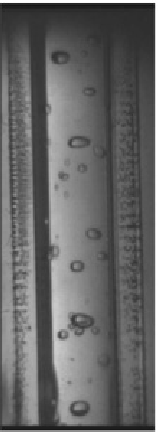
\includegraphics[width=1.1cm]{exp01.png}
        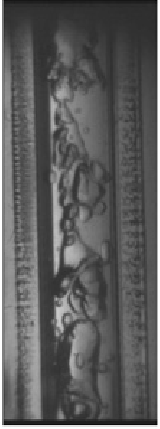
\includegraphics[width=1.1cm]{exp02.png}
        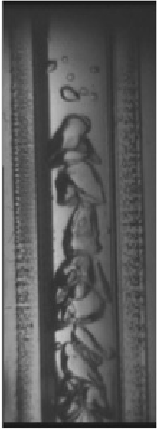
\includegraphics[width=1.1cm]{exp03.png}
        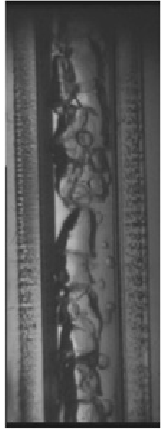
\includegraphics[width=1.1cm]{exp04.png}
        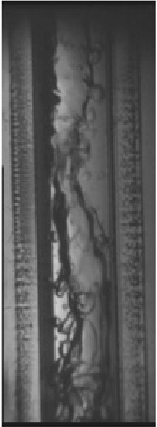
\includegraphics[width=1.1cm]{exp05.png}
        \caption{Flow Boiling Regimes~\footnotemark}
        \label{fig:self}
      \end{figure}
    \end{column}
  \end{columns}
  \footnotetext{\tiny \bibentry{baldassari2012flow}}
\end{frame}

\begin{frame}
  \frametitle{Motivation II}
  \begin{block}{Why microchannels are different?}
    \begin{itemize}
    \item $\Uparrow$ viscosity, diffusion, surface tension, contact lines
    \item $\Downarrow$ gravity, inertia
    \end{itemize}
  \end{block}

  \begin{block}{Viscosity}
    $1<\text{Re}<2000$ $\implies$ full Navier-Stokes (NS) equations~\footnotemark
  \end{block}
  \footnotetext{\tiny \bibentry{worner_numerical_2012}}
\end{frame}

\begin{frame}
  \frametitle{Models}
  \begin{itemize}
  \item VOF \\
    \bibintext{welch_local_1995}, \\
    \bibintext{kunkelmann_cfd_2009}
  \item Lattice Boltzmann \\
    \bibintext{markus_pool_2012}
  \item Particle-Based \\
    \bibintext{muller_particle-based_2005}, \\ 
   \bibintext{yoon_direct_2001}
  \end{itemize}
\end{frame}

%%% Local Variables: 
%%% mode: latex
%%% TeX-master: t
%%% End: 
